% !TEX encoding = UTF-8
% !TEX TS-program = pdflatex
% !TEX root = ../tesi.tex
% !TEX spellcheck = it-IT

%**************************************************************
\chapter{Conclusioni}
\label{cap:conclusioni}
Lo scopo principale dello stage era valutare se i prototipi precedentemente realizzati, in collaborazione con un processo d'elaborazione lato server che sfruttasse le potenzialità della libreria PCL, potessero essere migliorati fino ad ottenere un applicativo, inseribile nel contesto produttivo aziendale, da utilizzare del campo ispettivo. 
I risultati ottenuti sono stati piuttosto soddisfacenti, e quanto realizzato, anche se definito ancora allo stadio prototipale, una volta applicate le necessarie migliorie e raffinamenti, potrà diventare un'applicazione completa di grande utilità nel contesto sopracitato.

%**************************************************************
\section{Prove pratiche di calcolo del volume}
Uno degli obiettivi di primaria importanza del progetto, passo finale del processo di elaborazione e meshing di un Point Cloud, era il calcolo del volume dell'oggetto scansionato, che è uno dei parametri di valutazione del processo ispettivo.
Per rendere l'applicazione utilizzabile nel contesto produttivo è necessario che il calcolo del volume si discosti il meno possibile dal volume reale dell'oggetto. 
Vediamo ora nelle tabelle \ref{tab:calcolo-cestino} e \ref{tab:calcolo-scatola} i risultati ottenuti con l'applicativo nella sua ultima versione, per poi discuterne la bontà ed analizzare meglio il problema.
\subsection{Calcolo del volume di un cestino}
\begin{itemize}
\item \textbf{Oggetto}: Cestino cilindrico
\item \textbf{Volume reale}: 0.5652 $ m^3 $
\end{itemize}
\LTXtable{\textwidth}{tabelle/calcoloVolumeCestino.tex}
\begin{tabular}{l r}
\textbf{Volume medio}: 0.453 $m^3$ & \hspace{115pt} \textbf{Errore medio}: 19.94\% \\
\end{tabular}
\newline

\noindent
I risultati del primo set di test, effettuati scansionando un cestino di forma (approssimativamente) cilindrica non sono particolarmente buoni. L'errore medio del calcolo si assesta infatti attorno al 20\%, con picchi di errore del 42\%. Tali valori sono inaccettabili per un utilizzo produttivo dell'applicativo. La causa principale di tale divergenza è da ricercarsi nella scarsa qualità dei Point Cloud ricostruiti, che soffrivano di evidenti problemi di \emph{drifting}, complice anche la lucidità della superficie metallica del cestino, causa di disturbo al sensore di profondità infrarosso.

\subsection{Calcolo del volume di una scatola}
\begin{itemize}
\item \textbf{Oggetto}: Scatola 
\item \textbf{Volume reale}: 0.42 $ m^3 $
\end{itemize}
\LTXtable{\textwidth}{tabelle/calcoloVolumeScatola.tex}
\noindent
\begin{tabular}{l r}
\textbf{Volume medio}: 0.451 $m^3$ & \hspace{115pt} \textbf{Errore medio}: 14.74\% \\
\end{tabular}
I risultati del secondo set di test, effettuati scansionando una scatola di forma parallelepipoidale, sono molto migliori di quanto osservato nei primi test.
L'errore medio del calcolo si assesta infatti attorno al 14.7\%, anche se la bontà della media è ampiamente sfalsata da un paio di risultati particolarmente erronei, mentre i restanti 8 test riportano un errore inferiore al 10\%.
I Point Cloud ricostruiti della scatola erano molto più accurati di quelli del cestino, di qui i risultati migliori, anche se le ricostruzioni soffrivano ancora parzialmente di problemi di \emph{ghosting} e \emph{drifting}.

\subsection{Conclusioni sul calcolo del volume}
Analizzando i dati raccolti risulta evidente che l'applicazione non è ancora pronta per un uso affidabile sul campo. L'esito del calcolo è strettamente correlato alla qualità della mesh da valutare, quindi dal Point Cloud del quale si effettua il meshing e, risalendo alla radice, alla qualità del Point Cloud inizialmente ricostruito.\\
Per essere utilizzabile in un contesto produttivo l'applicativo deve generare stime il cui errore dev'essere sufficientemente basso (ad es. $\leq$ 5\%), e per ottenere tale risultato è necessario migliorare prima di tutto la ricostruzione iniziale dell'oggetto, come già tentato e discusso nella sezione "\emph{JNI e Point Cloud Registration}" (sez. \ref{sec:registration}).


%**************************************************************
\section{Problemi irrisolti e sviluppi futuri}
Il progetto è nato in tempi molto recenti, dopo circa tre mesi di sviluppo sono stati
prodotti più di un prototipo soddisfacente, l'ultimo dei quali realizzato dal tirocinante. La natura sperimentale del progetto ha fatto emergere durante la realizzazione una serie di problemi spesso non banali, alcuni dei quali irrisolti, ma anche una serie di idee e funzionalità per migliorare l'applicativo. Riporto di seguito alcuni di entrambe le categorie.
\subsection{Problemi irrisolti}
\subsubsection{Artefatti nel Point Cloud}
Durante l'acquisizione dei Point Cloud necessari a ricostruire l'oggetto scansionato, capita spesso che l'acquisizione sia disturbata da alcuni "artefatti", cioè gruppi di punti, tipicamente porzioni di piano, che non hanno corrispettivo nel mondo reale, e degradano la qualità della ricostruzione. Ne vediamo un esempio in figura \ref{fig:artefatti}.
\begin{figure}[!h] 
    \centering 
    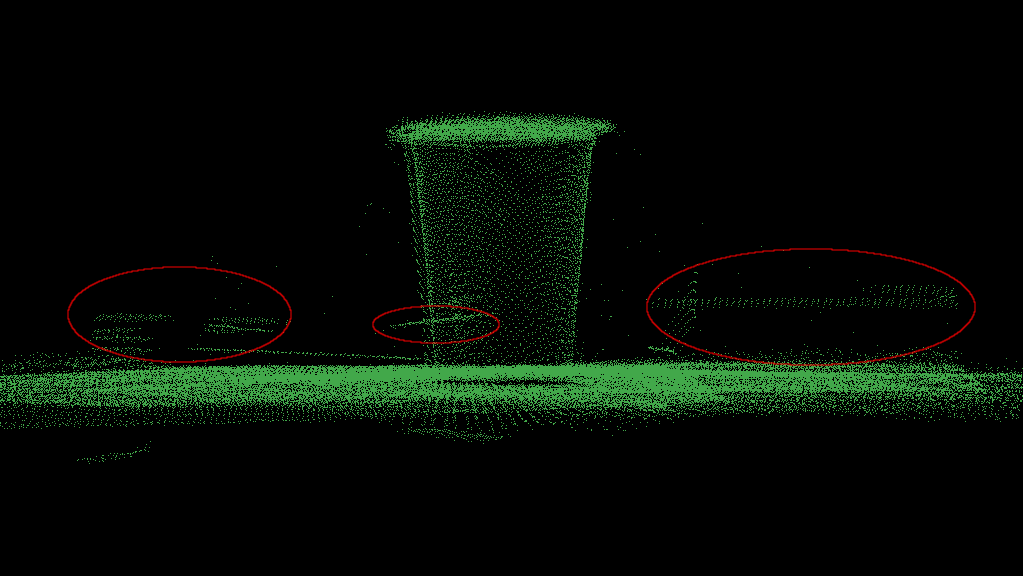
\includegraphics[width=1.0\columnwidth]{varie/artefatti.png} 
    \caption{Esempio di artefatti in un Point Cloud}
   \label{fig:artefatti}
\end{figure}
\newline
L'origine di tali artefatti non è ancora chiara, tra le possibili cause ipotizzate:
\begin{itemize}
\item Un bug nascosto nell'acquisizione dei punti
\item La presenza di riflessi sulle superfici scansionate, che causano problemi al sensore di profondità
\item Problemi di esposizione della fotocamera RGB
\end{itemize}
\noindent
Solitamente gli artefatti possono essere eliminati con successo attraverso il filtraggio \emph{Cluster extraction}, ma capita talvolta che un artefatto vada ad intersecare i punti dell'oggetto scansionato, rendendo così impossibile estrarre una nuvola di punti che rappresenti precisamente l'oggetto.

\subsubsection{Surriscaldamento e consumo della batteria}
Il \emph{device Tango} è sottoposto ad un notevole sforzo computazionale durante l'acquisizione dei Point Cloud, a causa dell'utilizzo di più sensori e di pesanti elaborazioni parallele, ed è facilmente predisposto al surriscaldamento (che ne peggiora le prestazioni) e ad un consumo eccessivo della batteria. Non era negli scopi dello stage affrontare tali problematiche, ma in un futuro potrebbe essere necessario risolverle rendendo più performante il processo di aquisizione.

\subsubsection{Drift correction???}

\subsection{Sviluppi futuri}

\subsubsection{Point Cloud Registration}

\subsubsection{Comparazione con modello 3D esatto}

\subsubsection{Miglioramento server}

\subsubsection{Integrazione con VIC}

\subsubsection{Meshing con textures}

%**************************************************************
\section{Consuntivo finale}

%**************************************************************
\section{Raggiungimento degli obiettivi}

%**************************************************************
\section{Conoscenze acquisite}

